Задача распределения фильмов по странам, в которых данные фильмы были сняты, позволяет получить представление о количестве фильмов, которые были сняты в конкретной стране, а также выделить те из них, количество снятых фильмов у которых наибольшее. 
Для реализации этой задачи используется информация из блока общих данных (Рис.~\ref{fig:1}), а именно иформация о странах, снявших конкретный фильм. Далее происходит суммирование полученной информации и сортировка в порядке убывания. 
Итогом работы является таблица, в которой отображены названия стран и соответствующие им значения снятых фильмов.
Для удобства визуализации выбраны первые 15 позиций.

\begin{figure}[ht!]
	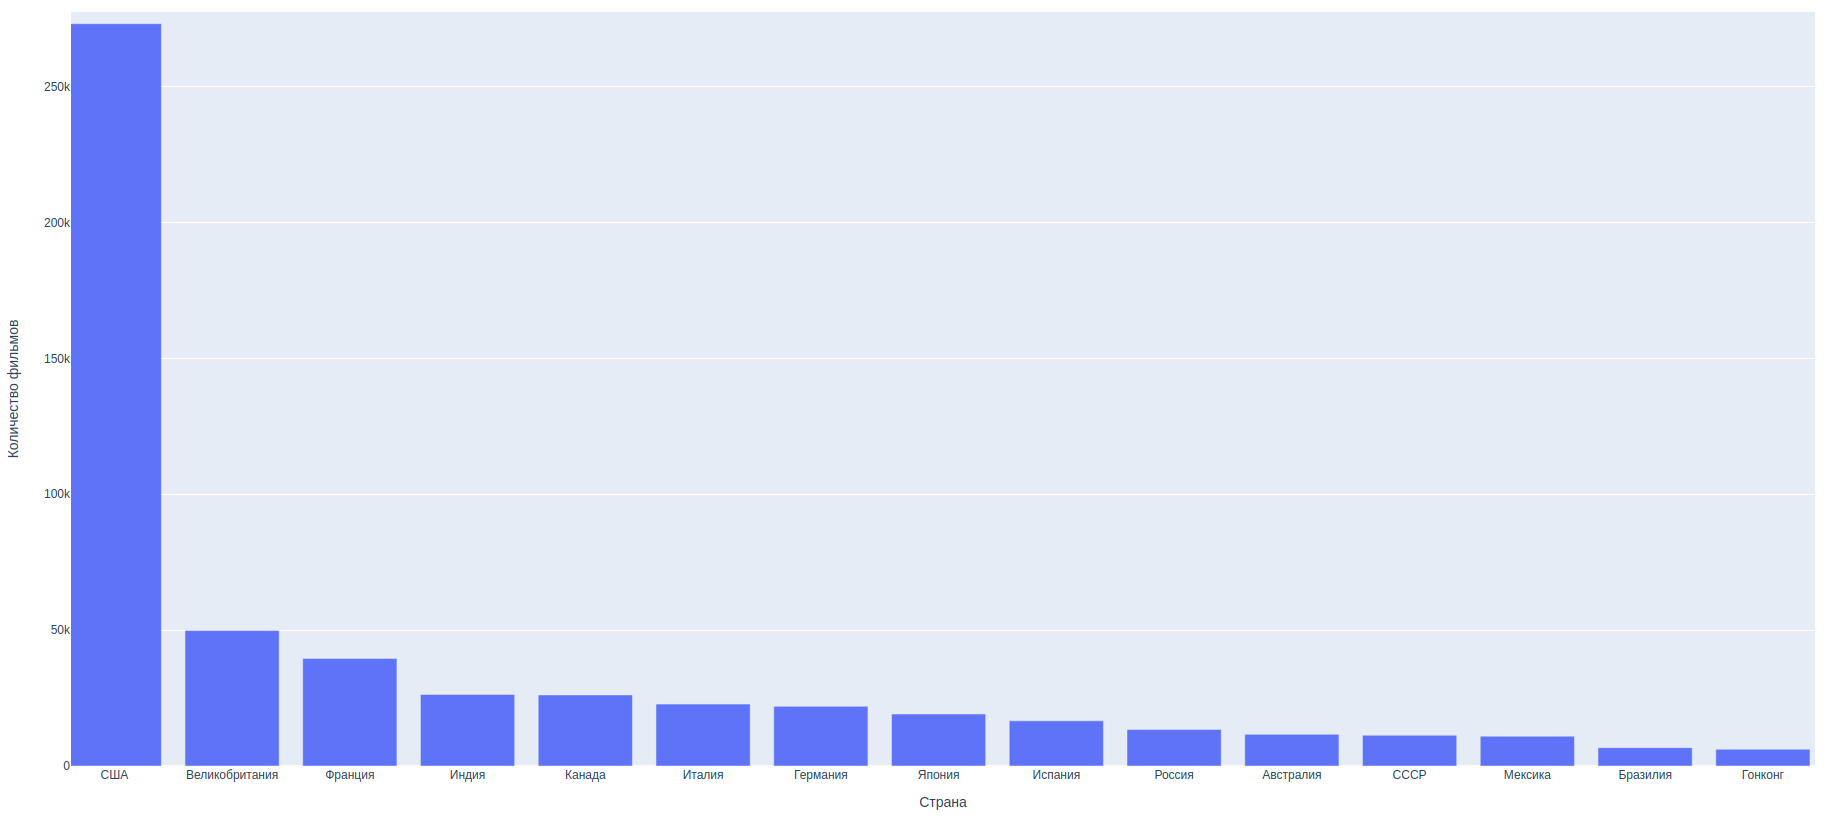
\includegraphics[width=\linewidth]{../report/images/films_by_country/2}
	\caption{Количество фильмов, снятых в конкретных странах}
	\label{fig:films_by_country_task}
\end{figure}

Представленный на Рис.~\ref{fig:films_by_country_task} график демонстрирует, что первенство по количеству снятых фильмов с огромным отрывом достается США, второе и третье место занимают Великобритания и Франция соответственно.